% !TEX encoding = UTF-8
% !TEX TS-program = pdflatex
% !TEX root = ../tesi.tex

%**************************************************************
\chapter{L'azienda}
\label{cap:azienda}
%**************************************************************
\section{Introduzione}

\vspace{20pt}
  \begin{figure}[!ht]
    \begin{center}
      
\includegraphics[width=6cm]{logo-wavelop}
      \caption{Logo azienda Wavelop S.R.L.S}
      \textbf{Fonte:} \href{https://www.wavelop.com}{wavelop.com}
    \end{center}
  \end{figure}
\vspace{20pt} 

Wavelop è un’azienda giovane e innovativa, con sede operativa a Treviso e sede legale a Venezia, che si occupa dello \
sviluppo di applicazioni web e \emph{mobile} per \emph{startup} e imprese. L’ambiente è informale e dinamico, con un focus \
alla flessibilità e al lavoro da remoto. \\

L’azienda riesce a soddisfare le richieste dei clienti grazie all’utilizzo della metodologia Agile Scrum ed \
alla creazione di \emph{design user-centered}, realizzando \emph{\gls{mock-up}} e prototipi per ottenere i risultati più adatti. \
Vengono, inoltre, utilizzate le migliori tecnologie in base al progetto richiesto.

%**************************************************************
\section{Tecnologie utilizzate}

\subsection{\emph{\Gls{backend}}}

\begin{itemize}
  \item \textbf{\emph{TypeScript}}: linguaggio basato su JavaScript, sviluppato da Microsoft, al quale viene aggiunta \
  la definizione statica dei tipi. Tutto ciò porta ad un rischio minore di \emph{bugs};
  \item \textbf{\emph{Node.js}}: è un sistema \emph{runtime} per JavaScript orientato agli eventi asincroni, è progettato \
  per realizzare applicazioni di rete scalabili;
  \item \textbf{\emph{MongoDB}}: è un \emph{database} NoSQL \emph{document-oriented}, permette di sviluppare applicazioni \
  flessibili e che possono scalare facilmente;
  \item \textbf{Servizi \emph{\acrfull{aws}}}: sono i servizi \emph{cloud} forniti da Amazon che comprendono: \
  \emph{cloud-computing}, archiviazione, \emph{Machine-Learning} e \emph{Internet of Things}. L'azienda utilizza \
  principalmente: 
  \begin{itemize}
    \item AWS Lambda: computazione \emph{serverless};
    \item AWS DynamoDB: \emph{database} NoSQL;
    \item AWS API Gateway: creazione di \acrshort{api}.
  \end{itemize}
\end{itemize}

\subsection{\emph{\Gls{frontend}}}

\begin{itemize}
  \item \textbf{\emph{React}}: è una libreria \emph{\gls{open-source}} JavaScript per realizzare interfacce utente. Sfrutta \
  il principio dello sviluppo per componenti e aggiorna solo i componenti che dipendono dai dati che hanno subito una \
  variazione;
  \item \textbf{\emph{Vue}}: è un \emph{framework} JavaScript \emph{open-source}, orientato al \emph{design pattern} \
  \acrshort{mvvm}, che permette la realizzazione di interfacce utente e \emph{Single Page Application};
  \item \textbf{\emph{Angular}}: è un \emph{framework open-source} basato su TypeScript sviluppato da Google che permette \
  di realizzare applicazioni universali per \emph{desktop}, \emph{mobile} e \emph{tablet}.
\end{itemize}

%**************************************************************
\section{Processi aziendali}

\subsection{Metodologia Agile}
La metodologia Agile è un approccio iterativo al \emph{project management} che consente ai \emph{team} di sviluppo \
di consegnare al cliente il prodotto più rapidamente. In particolare, con lo sviluppo Agile, il \emph{team} si presta a \
lavorare su piccoli incrementi utilizzabili. Ci sono molteplici metodologie che fanno riferimento al \emph{"Agile Manifesto"}, la più diffusa, e utilizzata \
dall'azienda, è lo \emph{Scrum}. \\

Lo \emph{Scrum} è un \emph{framework} che incoraggia i membri del \emph{team} a lavorare insieme. È basato sul principio dell'apprendimento continuo e sull'adattamento a situazioni che cambiano continuamente, mediante ri-prioritizzazione dei processi e brevi cicli di rilascio, chiamati \textbf{Sprint}, che permettono al \emph{team} di imparare e migliorare. Nello \emph{Scrum} si identificano tre artefatti che sono in continuo aggiornamento durante il progetto:

\begin{itemize}
  \item \textbf{\emph{Product Backlog}}: è la lista dei \emph{tasks} che devono essere svolti e viene mantenuta dal \emph{Product Owner}. La lista contiene \emph{features}, requisiti, miglioramenti e correzioni che fungeranno da \emph{input} allo \emph{Sprint Backlog}. I \emph{tasks} presenti nella lista sono costantemente revisionati, mantenuti e, inoltre, possono subire un cambiamento di priorità; 
  \item \textbf{\emph{Sprint Backlog}}: è la lista dei \emph{tasks} selezionati durante l'incontro di pianificazione dello \emph{sprint}, dal \emph{team} di sviluppo, per lo svolgimento nello \emph{sprint cycle} corrente. Lo \emph{sprint backlog} può essere flessibile durante lo \emph{sprint}, ma lo \emph{sprint goal} da raggiungere non deve essere compromesso.
  \item \textbf{Incremento} (o \emph{Sprint Goal}): è il prodotto usabile realizzato durante lo \emph{sprint}. Solitamente viene effettuata una dimostrazione al cliente, attraverso una demo, per mostrare il prodotto realizzato durante lo \emph{sprint} e per ottenere \emph{feedbacks} sul lavoro svolto.
\end{itemize}

Nella pratica, lavorare con il \emph{framework Scrum}, significa svolgere le seguenti attività:
\begin{itemize}
  \item \textbf{\emph{Sprint Planning}}: l'intero \emph{team} di sviluppo si riunisce per definire l'obiettivo dello \emph{sprint} che si andrà a svolgere e vengono scelte le \emph{user stories} da spostare dal \emph{product backlog} allo \emph{sprint backlog} che dovranno essere coerenti con lo \emph{sprint goal};
  \item \textbf{\emph{Sprint}}: è un periodo di tempo, solitamente una o due settimane, durante il quale il \emph{team} implementa le \emph{user stories} presenti nello \emph{sprint backlog};
  \item \emph{\textbf{Daily Scrum} (o Stand up)}: sono delle velocissime riunioni giornaliere che durano circa 15 minuti, durante le quali il \emph{team} si allinea sul lavoro svolto e pianifica il lavoro della giornata. Tipicamente durante lo \emph{stand up meeting} ogni membro del \emph{team} deve rispondere alle seguenti tre domande: "Cosa ho fatto ieri?", "Cosa farò oggi?", "Ho avuto qualche problema?";
  \item \textbf{\emph{Sprint Review}}: è un incontro informale tra i membri del \emph{team} e gli \emph{\glspl{stakeholder}} per mostrare quali \emph{user stories}, presenti nello \emph{sprint backlog}, sono state completate e per ottenere dei \emph{feedbacks}. Inoltre il \emph{product owner} decide se rilasciare l'incremento o no;
  \item \textbf{\emph{Sprint Retrospective}}: è una riunione tra i membri del \emph{team} di sviluppo per discutere su cosa migliorare nel prossimo \emph{sprint} e su cosa ha funzionato nello \emph{sprint} appena concluso.
\end{itemize}

\clearpage

\vspace{20pt}
  \begin{figure}[!ht]
    \begin{center}
      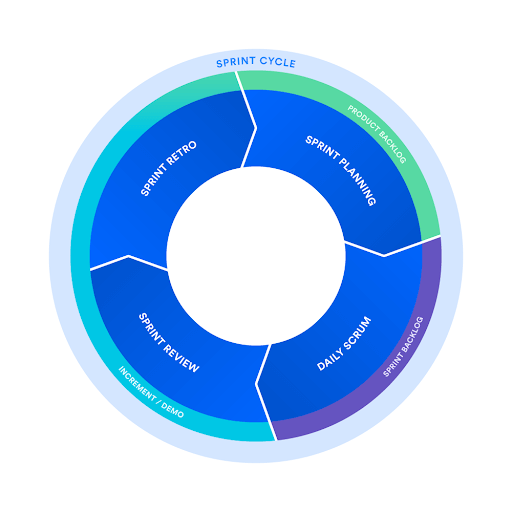
\includegraphics[height=12cm]{sprint-cycle}
      \caption{Ciclo di uno Sprint}
      \textbf{Fonte:} \href{https://www.atlassian.com}{atlassian.com}
    \end{center}
  \end{figure}
\vspace{20pt} 

\subsection{Strumeti a supporto dei processi}

\subsubsection{Git \& GitLab}
Git è un \emph{Distributed Version Control System}, \emph{open-source} e gratuito, progettato per gestire progetti di \
grandi e piccole dimensioni con efficienza. \\

GitLab, a differenza di git, è una piattaforma di \emph{hosting} per \emph{git repositories}; inoltre offre diversi servizi \
per la gestione del progetto, quali:

\begin{itemize}
  \item \emph{Issue Tracking System};
  \item \emph{Project Board}
  \item \emph{\acrfull{ci}};
  \item \emph{\acrfull{cd}}.
\end{itemize}

\vspace{20pt}
  \begin{figure}[!ht]
    \begin{center}
      
\includegraphics[height=3cm]{logo-gitlab}
      \caption{Logo GitLab}
      \textbf{Fonte:} \href{https://www.gitlab.com}{gitlab.com}
    \end{center}
  \end{figure}
\vspace{20pt} 

\subsubsection{\emph{Google Workspace}}
\emph{Google Workspace} è un insieme di strumenti di collaborazione e produttività sviluppato da Google. \
I servizi utilizzati maggiormente dall'azienda sono:

\begin{itemize}
  \item \emph{Gmail} per le comunicazioni formali;
  \item \emph{Calendar} per la gestione degli impegni aziendali;
  \item \emph{Drive} per la memorizzazione di file nel \emph{cloud};
  \item \emph{Meet} per le riunioni con i clienti;
  \item \emph{Google Docs Suite} per la creazione di documenti e presentazioni.
\end{itemize}

\vspace{20pt}
  \begin{figure}[!ht]
    \begin{center}
      
\includegraphics[width=10cm]{logo-google-workspace}
      \caption{Logo Google Workspace}
      \textbf{Fonte:} \href{https://workspace.google.com}{workspace.google.com}
    \end{center}
  \end{figure}
\vspace{20pt} 

%**************************************************************
\section{Rapporto con l'innovazione}
L'azienda è sempre aggiornata sulle nuove tecnologie partecipando ad incontri tecnologici con relatori di spicco: \emph{Google} e \emph{Amazon}, \
per citarne alcuni; in generale, è molto propensa all'innovazione accettando la presa in carico di progetti innovativi che sfruttano \
i moderni \emph{smart speakers}, l'architettura \emph{Serverless} o nell'ambito dell'\acrfull{iot}.